%\documentclass[runningheads,a4paper]{llncs}
\documentclass{article}

\usepackage{amssymb}
\setcounter{tocdepth}{3}
\usepackage{graphicx}
\usepackage{url}

\begin{document}

% \mainmatter 

\title{Autonomous Realization of Simple Machines}
\author{Can Erdogan \and Mike Stilman}
% \institute{Institute for Robotics and Intelligent Machines \\Georgia Institute of Technology}

\maketitle

\begin{abstract}

For robots to become integral parts of human daily experi- ence, they need to be able to utilize the
objects in their environment to accomplish any range of tasks. In this work, we focus particularly
on physically challenging tasks that push the limits on the robot kinodynamic constraints such as
joint limits, joint torques and etc. Previously, we demonstrated an autonomous planner that
instructs a human collab- orator where to place the available objects in the environment to form a
simple machine such as a lever-fulcrum assembly. In this work, we report results on the autonomous
realization of such a design by the humanoid robot Golem Krang, focusing on the challenges of
autonomous perception, manipulation and control.

\end{abstract}

\section{Introduction}

The ability to use the available objects in the environment towards accomplishing goals is essential
to thriving in challenging circumstances. Everyday examples of tool use include simple machines such
as levers and pulleys. The challenge in autonomous design of such simple machines is the space of
discrete choices for the component options and the related high-dimensional continuous configuration
space of the chosen components.

In previous work \cite{erdogan2013planning} \cite{erdogan2014incorporating}, we demonstrated the
constraint satisfaction approach to assembly design, specifically for robotic manipulation and
locomotion. The key idea is to represent the constraints
between the components of the design, the robot kinematics and dynamics as generic equality and
inequality functions within a nonlinear optimization framework and solve for the global minima, if
necessary by random restarts. Such global optimization methods have been used in other fields as
well, such as operations research \cite{vidal2006branching} and architecture \cite{yu2011make}.

In this work, we take the next step towards full autonomy where the humanoid robot, Golem Krang,
autonomously manipulates the objects in its environment to construct a simple machine. We present
an autonomous planner that perceives the available objects, specifically 15 kg cinder blocks and 10
kg 2-by-4 block blocks (e.g. potential levers), relocates them to the desired configurations output
by the constraint planner, and actuates them to flip a 45 kg load. Figure \ref{fig:showOff} demonstrates key scenes
from this scenario such as (a) detection of a cinder block, (b) locomotion with a heavy load, (c)
manipulating a lever while subject to multiple constraints and (d) application of force to the lever
leading to a successful load motion.

\begin{figure}[ht!] 
  \centering
  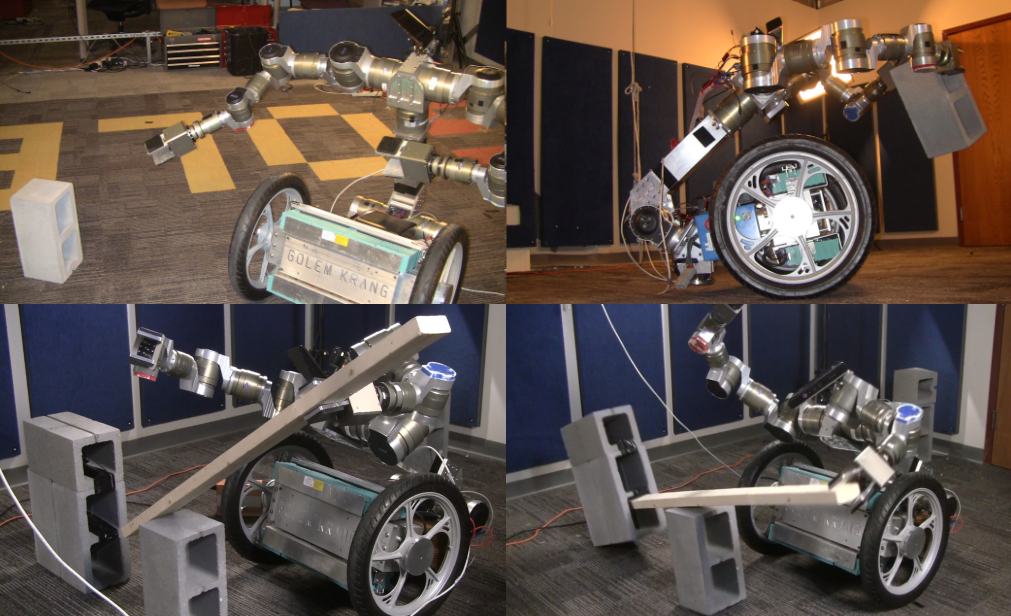
\includegraphics[width=1.0\linewidth]{Figures/showOff.png}
  \caption{The mechanical advantage in forces}
  \label{fig:showOff}
\end{figure}

Significant effort has been demonstrated by \cite{beetz2010cram} \cite{stilman2005navigation}
\cite{kemp2007challenges} to incorporate autonomous agents in human environments. Our work stands
out in multiple aspects from the established state of the art. First, Golem Krang is a two-wheeled
balancing robot, similar to a segway with two 7-dof robotic arms installed. The challenge with
such a platform is the dynamic stability constraint where the robot has to ensure its center of mass
is close to the wheel axis at all times as opposed to legged or multi-wheeled platforms. Secondly, to the best of our knowledge,
Golem Krang is the tallest and heaviest two-wheeled robot with 150 kg at 1.9 m, a unique property
among similar designs \cite{kuindersma2009dexterous}. As we expand in Section IV, at this scale, the
weight can help with heavy-duty manipulation but complicates the autonomous locomotion of the
agent. Lastly, Golem Krang perceives its environment with an onboard RGBD sensor with two degrees
of freedom that are manipulated autonomously for gaze control. Autonomous perception and scene
recognition has only recently started to gather interest in the humanoid robotics field
\cite{srinivasa2010herb} \cite{nishiwaki2000design} as opposed to the long established motion
capture methods \cite{dasgupta1999making}.

\section{Technical Approach}

We now present our approach to autonomous construction of simple machines, particularly a
lever-fulcrum assembly to overturn heavy obstacles, in four major categories: (1) autonomous design,
(2) visual perception, (3) posture control, and (4) motion planning.

In any design, components have to be placed to satisfy a set of physical or domain constraints. For
instance, a candidate 2-by-4 block needs to make contact both with the load and the fulcrum,
essentially distance functions between objects, to satisfy physical constraints of the design.
However, for a design to be useful, we also impose that the contact point for the lever is further
away from the fulcrum than the load such that a mechanical advantage is achieved. In previous work,
we propose a nonlinear optimization approach where such geometric and dynamic constraints are
expressed as equality and inequality functions whose common zero-crossings are design configurations
that satisfy all the constraints. For this work, we use the planner to output the lever and the
fulcrum configurations, and the required contact point, but allow the robot to choose its closest
configuration, assuming it can supply the necessary force.

In perceiving the environment, we propose using a light-weight feature-based recognition approach as
opposed to full 3D based approaches that use the entire mesh data such as the iterative closest
point algorithm or over-segmentation methods. The key assumption of the work is that the planner
already knows the mesh of the available objects and with minimal additional feature knowledge, such
as the top of a cinder block is at 44 cm from the ground or a lever is at least 2 meters in one
dimension, we can speed up detection. At its current stage, the agent can autonomously detect cinder
blocks, the load as shown in Figure 1, the walls and the 2-by-4 levers. To localize objects of
interest, we perform a simple scan with the tilt and pan degrees of freedom of the RGBD camera,
taking also into account the robot kinematics. Figure \ref{fig:detection} demonstrates the detection module.

\begin{figure}[ht!] 
  \centering
  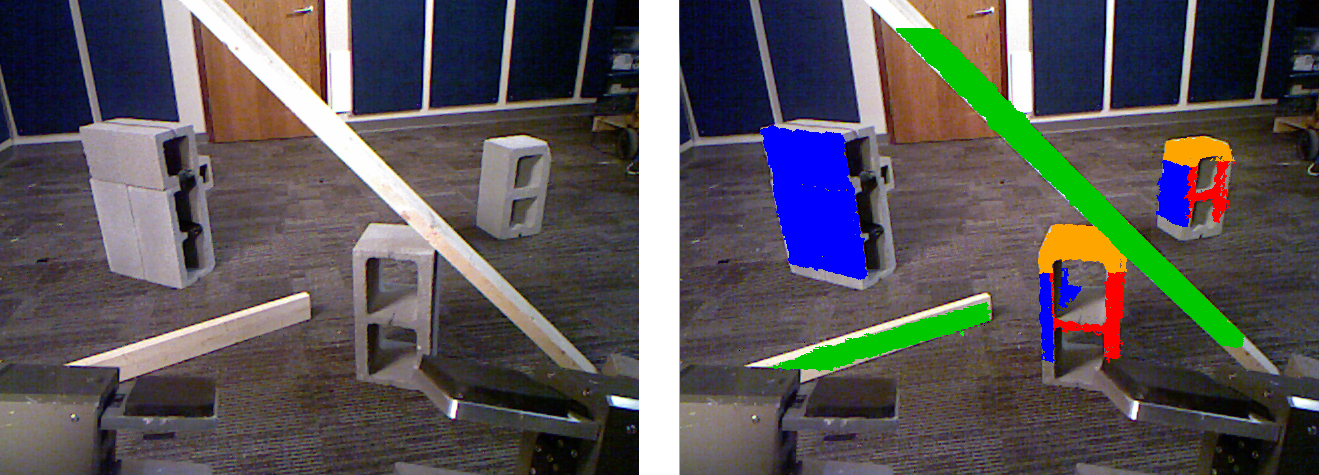
\includegraphics[width=1.0\linewidth]{Figures/detection.png}
  \caption{The mechanical advantage in forces}
  \label{fig:detection}
\end{figure}

For the locomotion controllers, we model Krang as a simple inverse pendulum and use a
proportional-derivative control with gain scheduling for different robot poses to minimize the
frequency of oscillations in dynamic balancing. In picking up cinder blocks, the torque around the
wheel axis due to the additional force at the end-effector is incorporated in computing the goal
balancing angle.

Lastly, for motion planning, we use a variety of approaches. First, to grasp objects, we use
analytical inverse kinematics to determine if there is a configuration close to the object we can
reach without collisions. Once close, we perform Jacobian inverse kinematics to approach the object
and detect contact with the object with the gripper force-torque sensor. Analytical inverse
kinematics is used as a resolution-complete method to determine whether a collision-free grasp
configuration exists as opposed to sampling the large configuration space of the arms to avoid local
minima with Jacobians. In addition to motion planning for the arms, we also make use of an example
of conformant planning in picking up a lever. The motivation is to avoid perception problems by
running each wheel to the 2-by-4 on the ground while the wheels cannot exert the torque to climb
over the object. Thus, the robot autonomously aligns itself with the object of interest by using
contact points without the need for precise perception.

\section{Results}

Our results demonstrate Golem Krang autonomously construct a simple machine design, specifically a
lever-fulcrum assembly, and use it to overturn a 45 kg load. To achieve such an autonomous behavior,
we propose a set of modules that accomplish object detection and localization, balancing and
navigation controller in the presence of external disturbances, and a rich set of motion planning
modules. To demonstrate the execution of the task, we designed the following scenario (see
\url{http://tinyurl.com/mw2ehxl} for video):

We position Golem Krang in the middle of the room and instruct it to use the closest cinder block as
a fulcrum. Using the aforementioned tools, the robot picks up the object (e.g. reacts to its weight
by leaning backwards) and carries it to the predetermined position instructed by the constraint
optimization planner. During locomotion, we assume that there are no obstacles on the path of the
robot, and the robot uses the turn-forward-turn tactic to move between two planar poses. Once the
robot places the fulcrum, it scans its surroundings for a lever and once located, approaches it
using the perception data. To minimize the effect of perception errors, once within 0.5 meters of
the lever, the robot deploys the wheel contact approach to position itself exactly in front of the
object and takes it back to the load. Finally, the robot positions the lever with Jacobian control
and exerts force with the top joint in its 7-dof arm.

\section{Experiments}

A significant challenge in accomplishing the series of the autonomous manipulation and perception
tasks has been the accumulation of error over the course of the executions. To remedy such an error
build-up, at the current state of our work, the authors intervene and instruct the robot to minimize
its position errors. We focus on the two main reasons and propose possible solutions.

During experiments, we observed that the RGBD data becomes more erroneous as the distance increases.
Within a 1 meter bound, the mean error is within 2-3 cm whereas with the maximum 4 meters (e.g. the
room limits), we see errors up to 10 cm. The proportional increase of error with respect to distance
suggest a camera calibration problem. Another source of error could be the slack in the tilt and pan
joints that control the camera view. The general of camera calibration has been addressed via bundle
adjustment in [2].

A second reason we suspect that might lead to localization errors is the error accumulated while the
robot attempts to follow a velocity profile in the forward direction. Figure \ref{fig:controller} demonstrates the
reference position and velocity trajectories (green), along with the real trajectories (red). To
remedy this error, we will focus on the trajectory following techniques developed by [7].

\begin{figure}[ht!] 
  \centering
  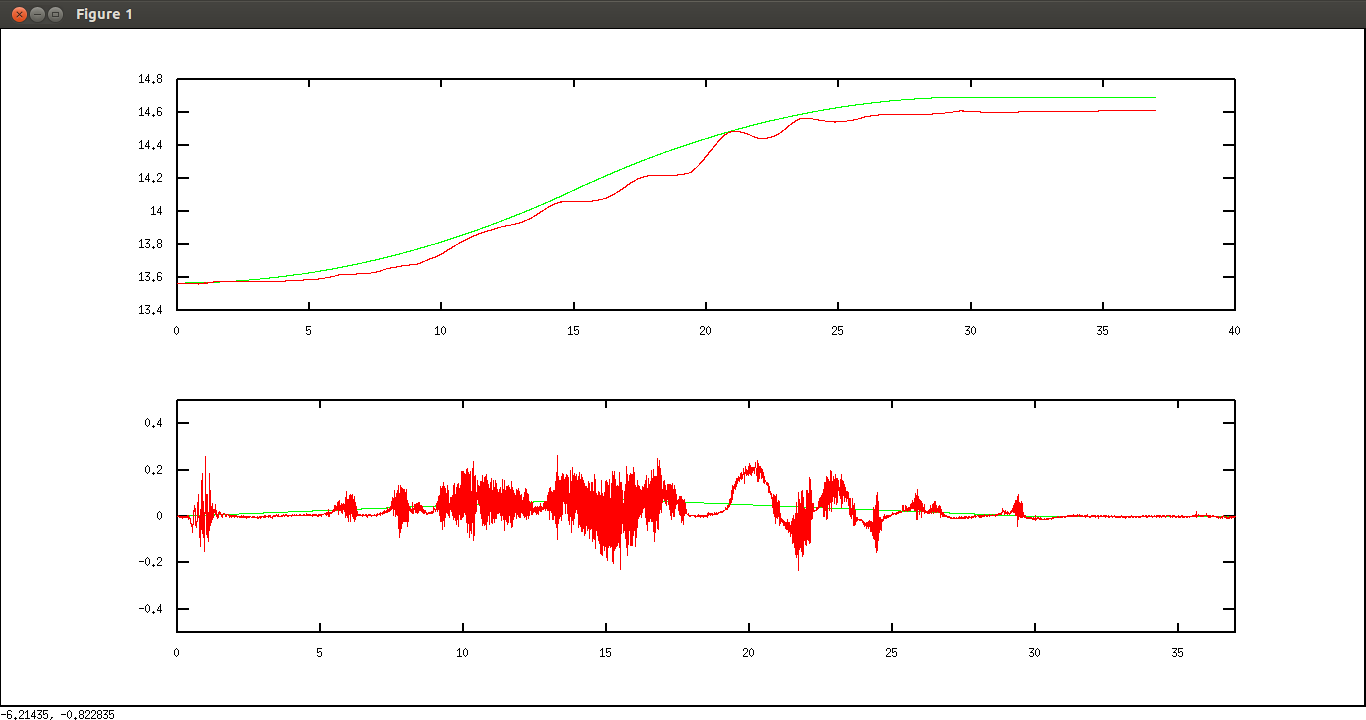
\includegraphics[width=0.6\linewidth]{Figures/controller.png}
  \caption{The mechanical advantage in forces}
  \label{fig:controller}
\end{figure}

Lastly, the main experiment of our work is the successful overturning of the 45 kg obstacle. Figure
4 demonstrate the forces measured at the robot gripper as it pushes the lever until the obstacle
falls. Given that the load is approximately 500N and the maximum force is 250N, we observe an
advantage of 2:1.

\begin{figure}[ht!] 
  \centering
  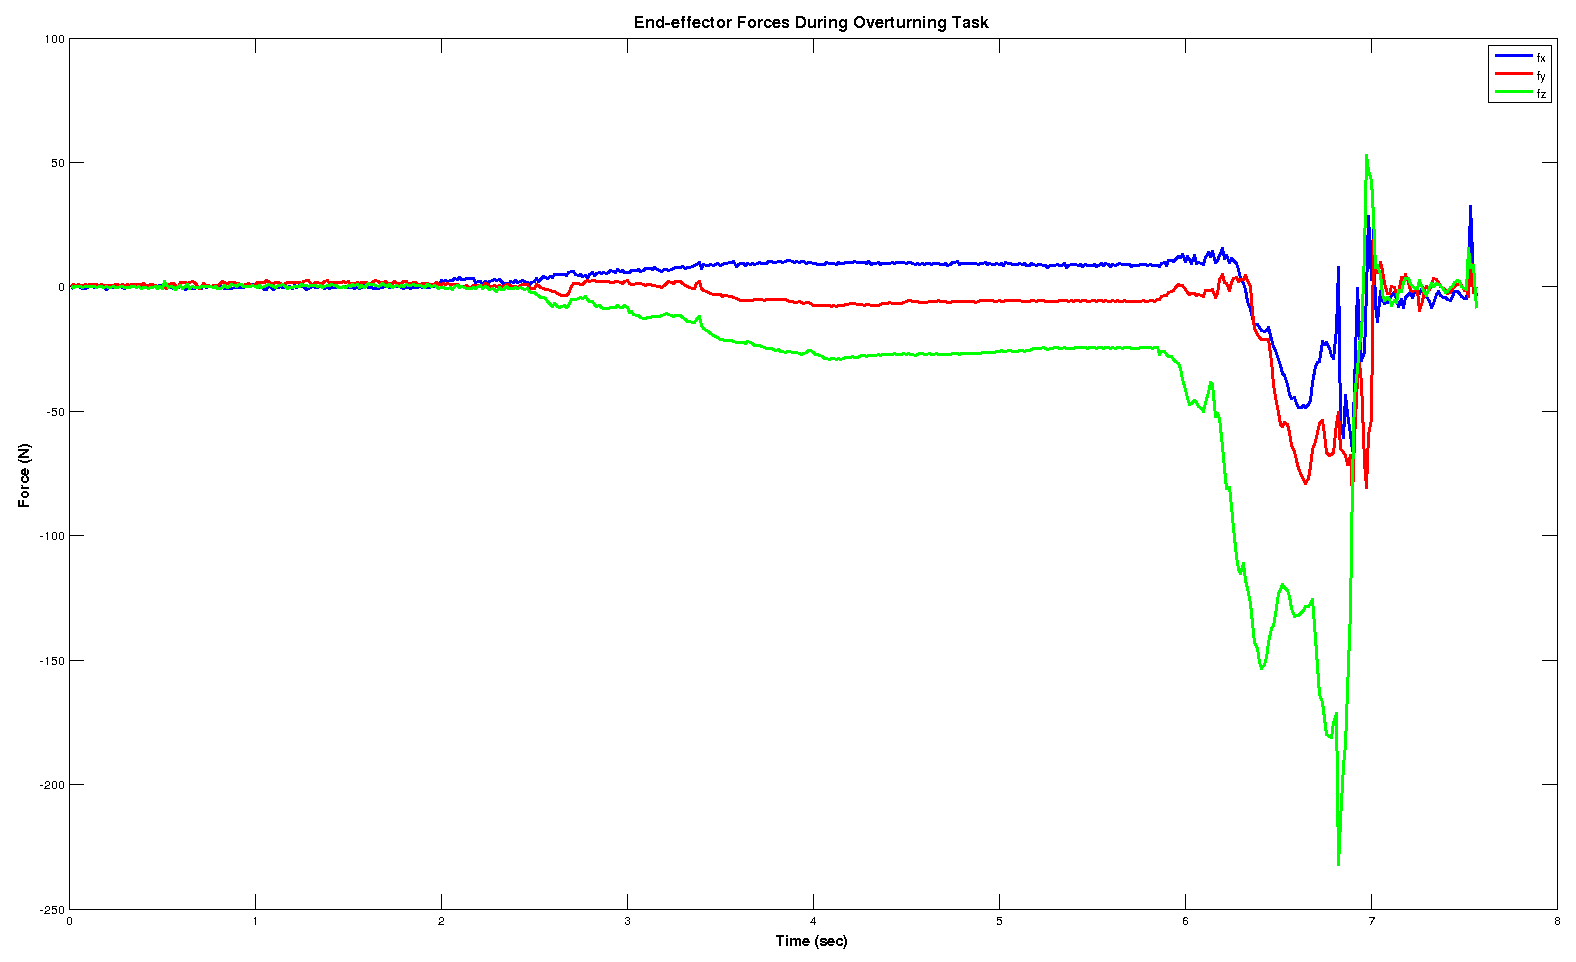
\includegraphics[width=0.6\linewidth]{Figures/plot.png}
  \caption{The mechanical advantage in forces}
  \label{fig:plot}
\end{figure}

\section{Experimental Insights}

We offer two insights from our experiments. First, the manipulation of heavy objects brings about
interesting challenges. If the object inertia model is not known, the system can be thrown off
balance easily. Moreover, when the mass of the object is mostly on one of the wheels, the robot can
start spinning since one wheel has to accommodate the extra weight. Second, the constraint
optimization planner outputs too precise (e.g. 1$e^{-5}$) configurations which we observe clearly
cannot be executed to the same level of precision. We propose extending the planner for iterative
solutions and/or soft constraints.


\bibliographystyle{plain}
\bibliography{references}

\end{document}
